% !TEX root = ../../thesis.tex

\section{ Aesthetic design of the head } % (fold)
\label{sec:head-design}
A lot of effort has been put into the design and aesthetic of Poppy's head (see \figurename~\ref{fig:poppy_beta_head}) because it is both its identity and main communication apparatus.
From an aesthetic point of view, its design was inspired of course by existing robots, but also by animals, objects and art. Insights into our  main inspirations are displayed on the board in \figurename~\ref{fig:head_inspiration}. We tried to achieve a design that is cute, expressive and above all, simple.

\begin{figure}[p]
    \begin{center}
        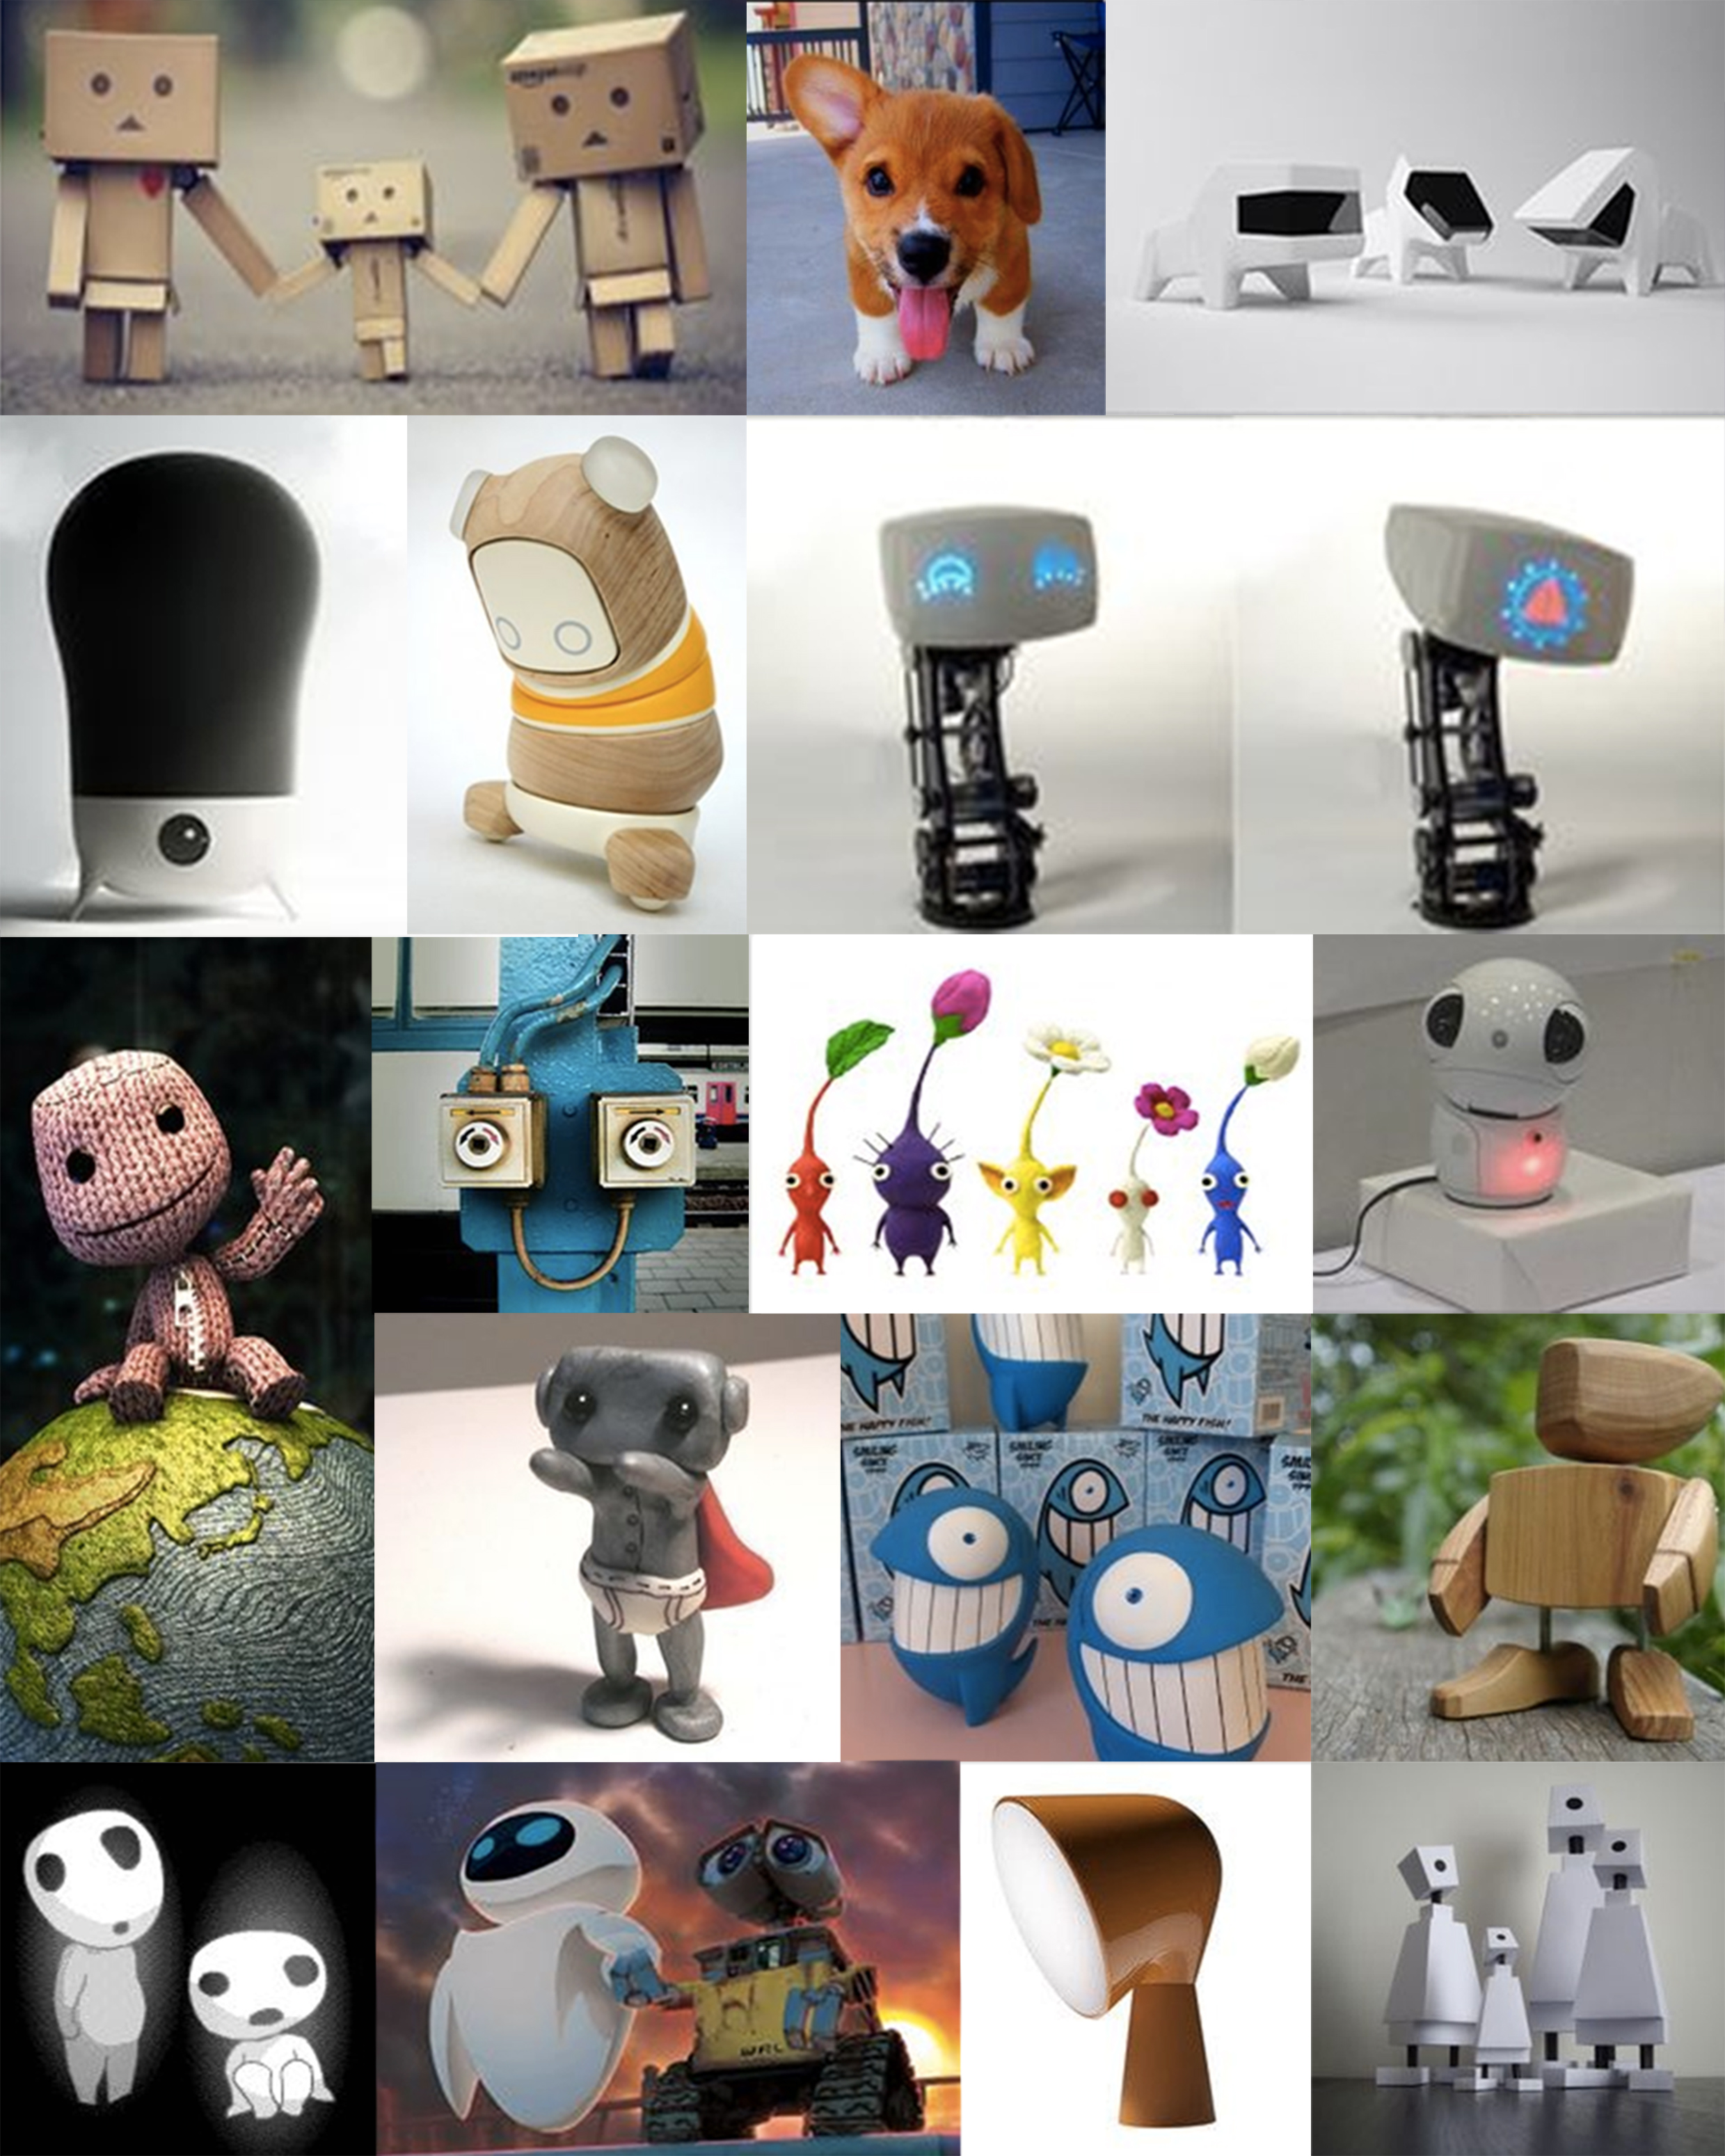
\includegraphics[width=\linewidth]{head_inspiration.jpg}
    \end{center}
    \caption{Complete board available on pinterest \url{http://www.pinterest.com/matthieulapeyre/robot/}}
    \label{fig:head_inspiration}
\end{figure}

Yet because of the multi-articulated vertebral column, there is only free room in Poppy’s head to embed all electronics components needed. Therefore strong technical constraints were imposed because all electronic architecture plus the communication sensorimotor apparatus composed by a wide 4.3" screen, cameras, and audio devices all have to be embedded in the head.
These components strongly constrained the design of the robot. Especially the screen, which necessitated a large flat part on the face. Obtaining a nice, rounded head shape with such constraints was rather difficult and require several iterations before obtaining the first correct finished version (see \figurename~\ref{fig:poppy_beta_head}).

This process firstly involved several sketches showing the main ideas of the desired design. But the transfer to CAD modelling was quite complex; these kinds of shape are rather difficult to design using parametric tools. The use of clay sculpting was very helpful  in the transition from the 2D drawing to the 3D shape.

\begin{figure}[p]
\centering
    \subfloat[][]{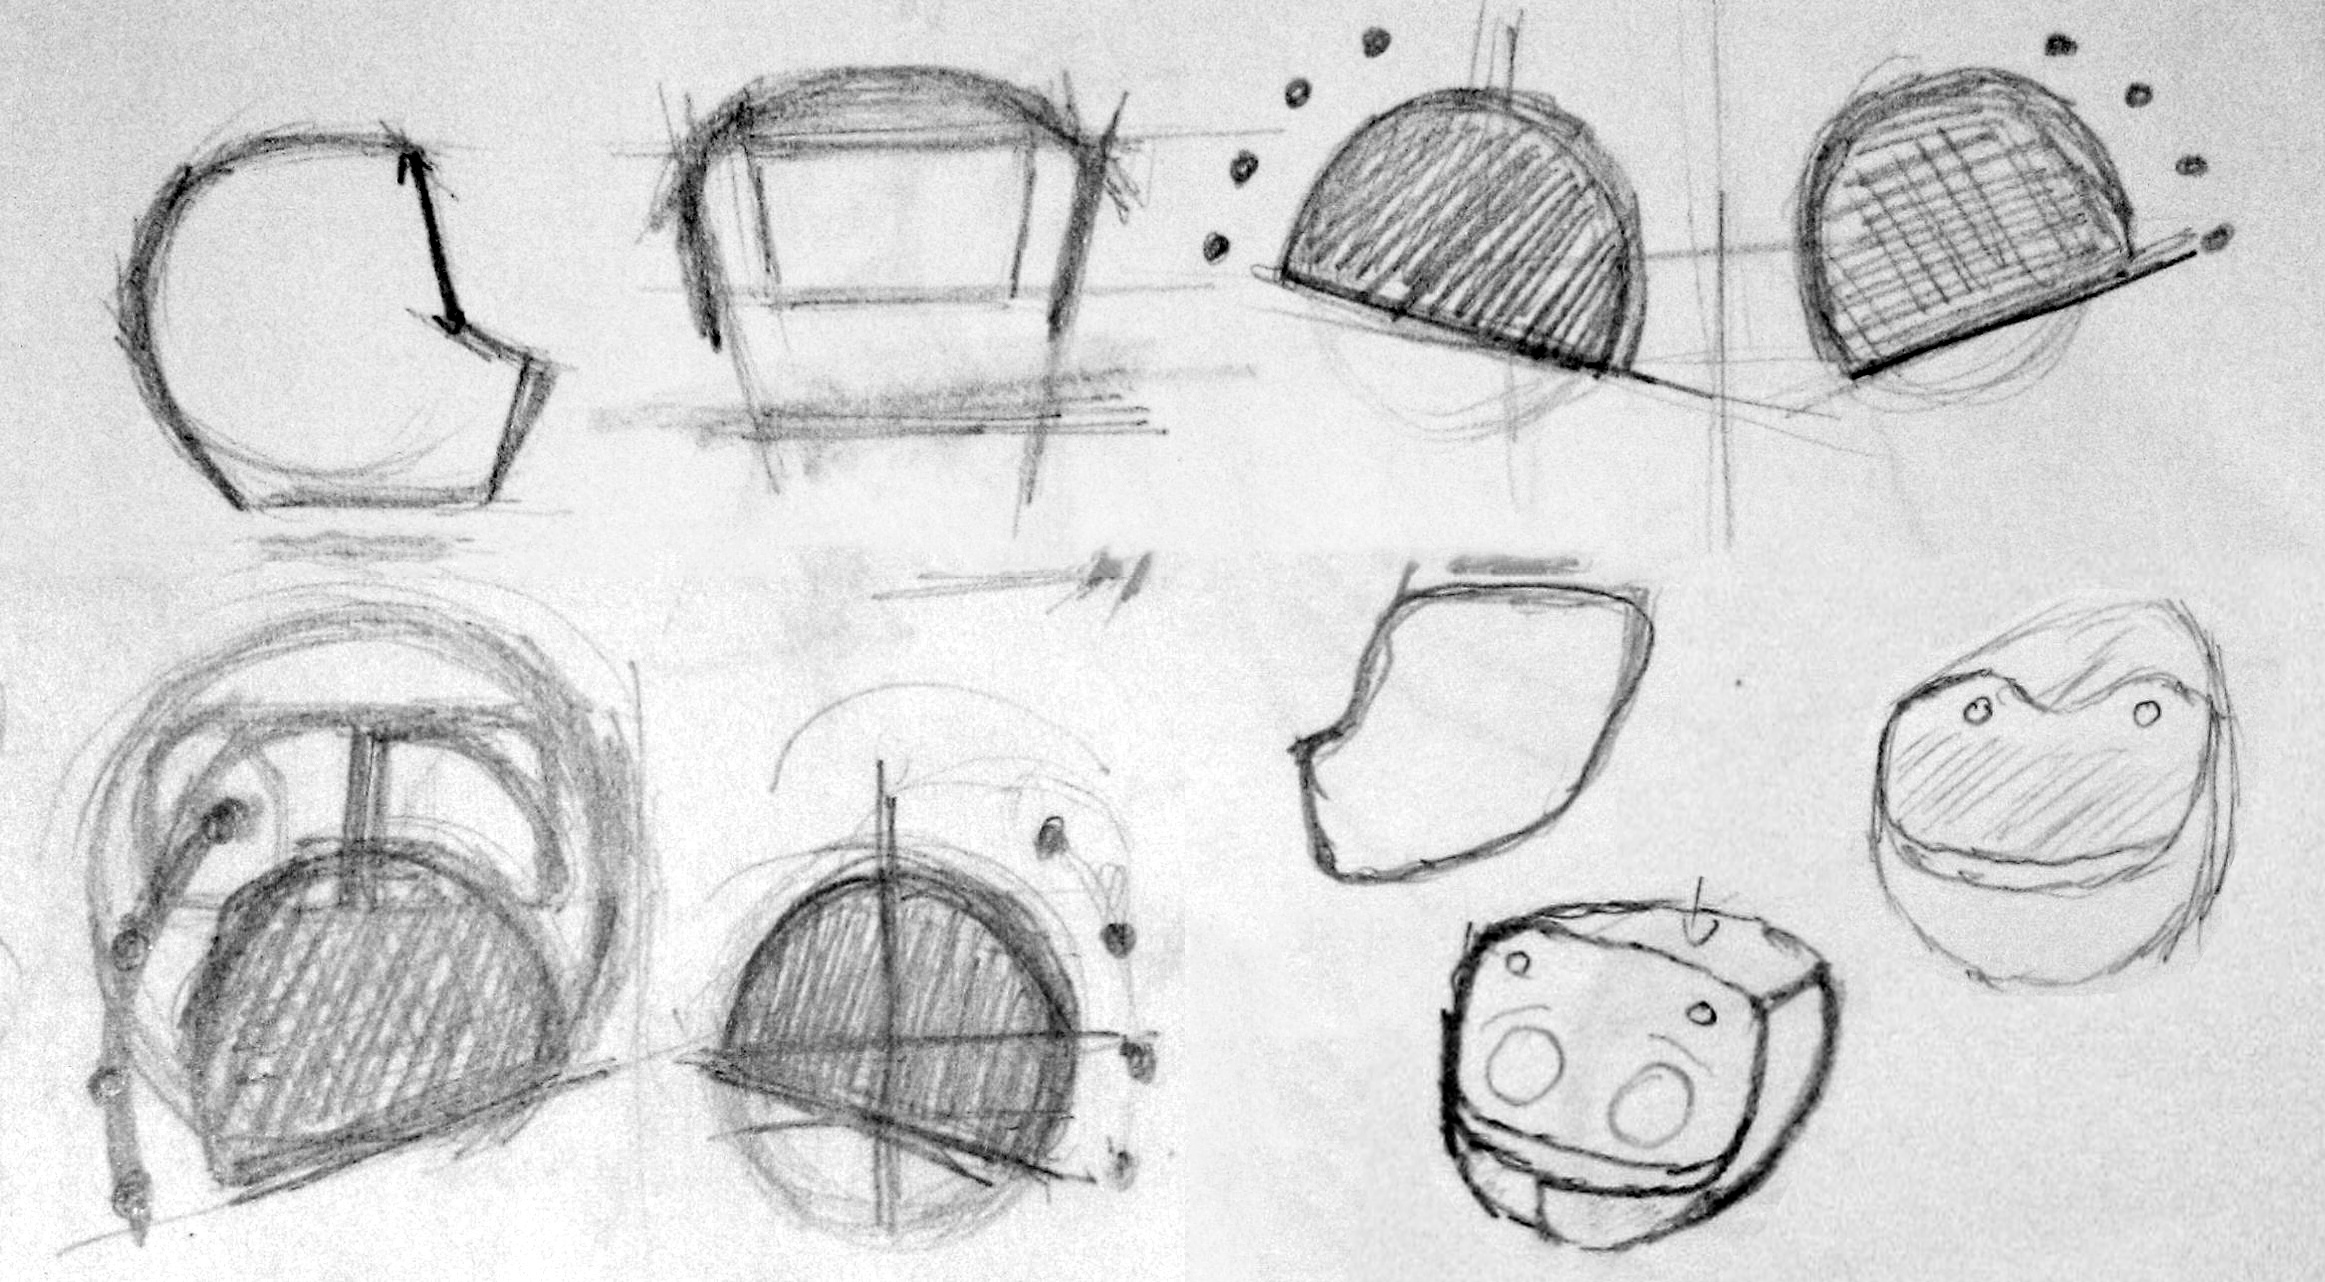
\includegraphics[height=4.5cm]{first_sketch.jpg}}
    \hfil
    \subfloat[][]{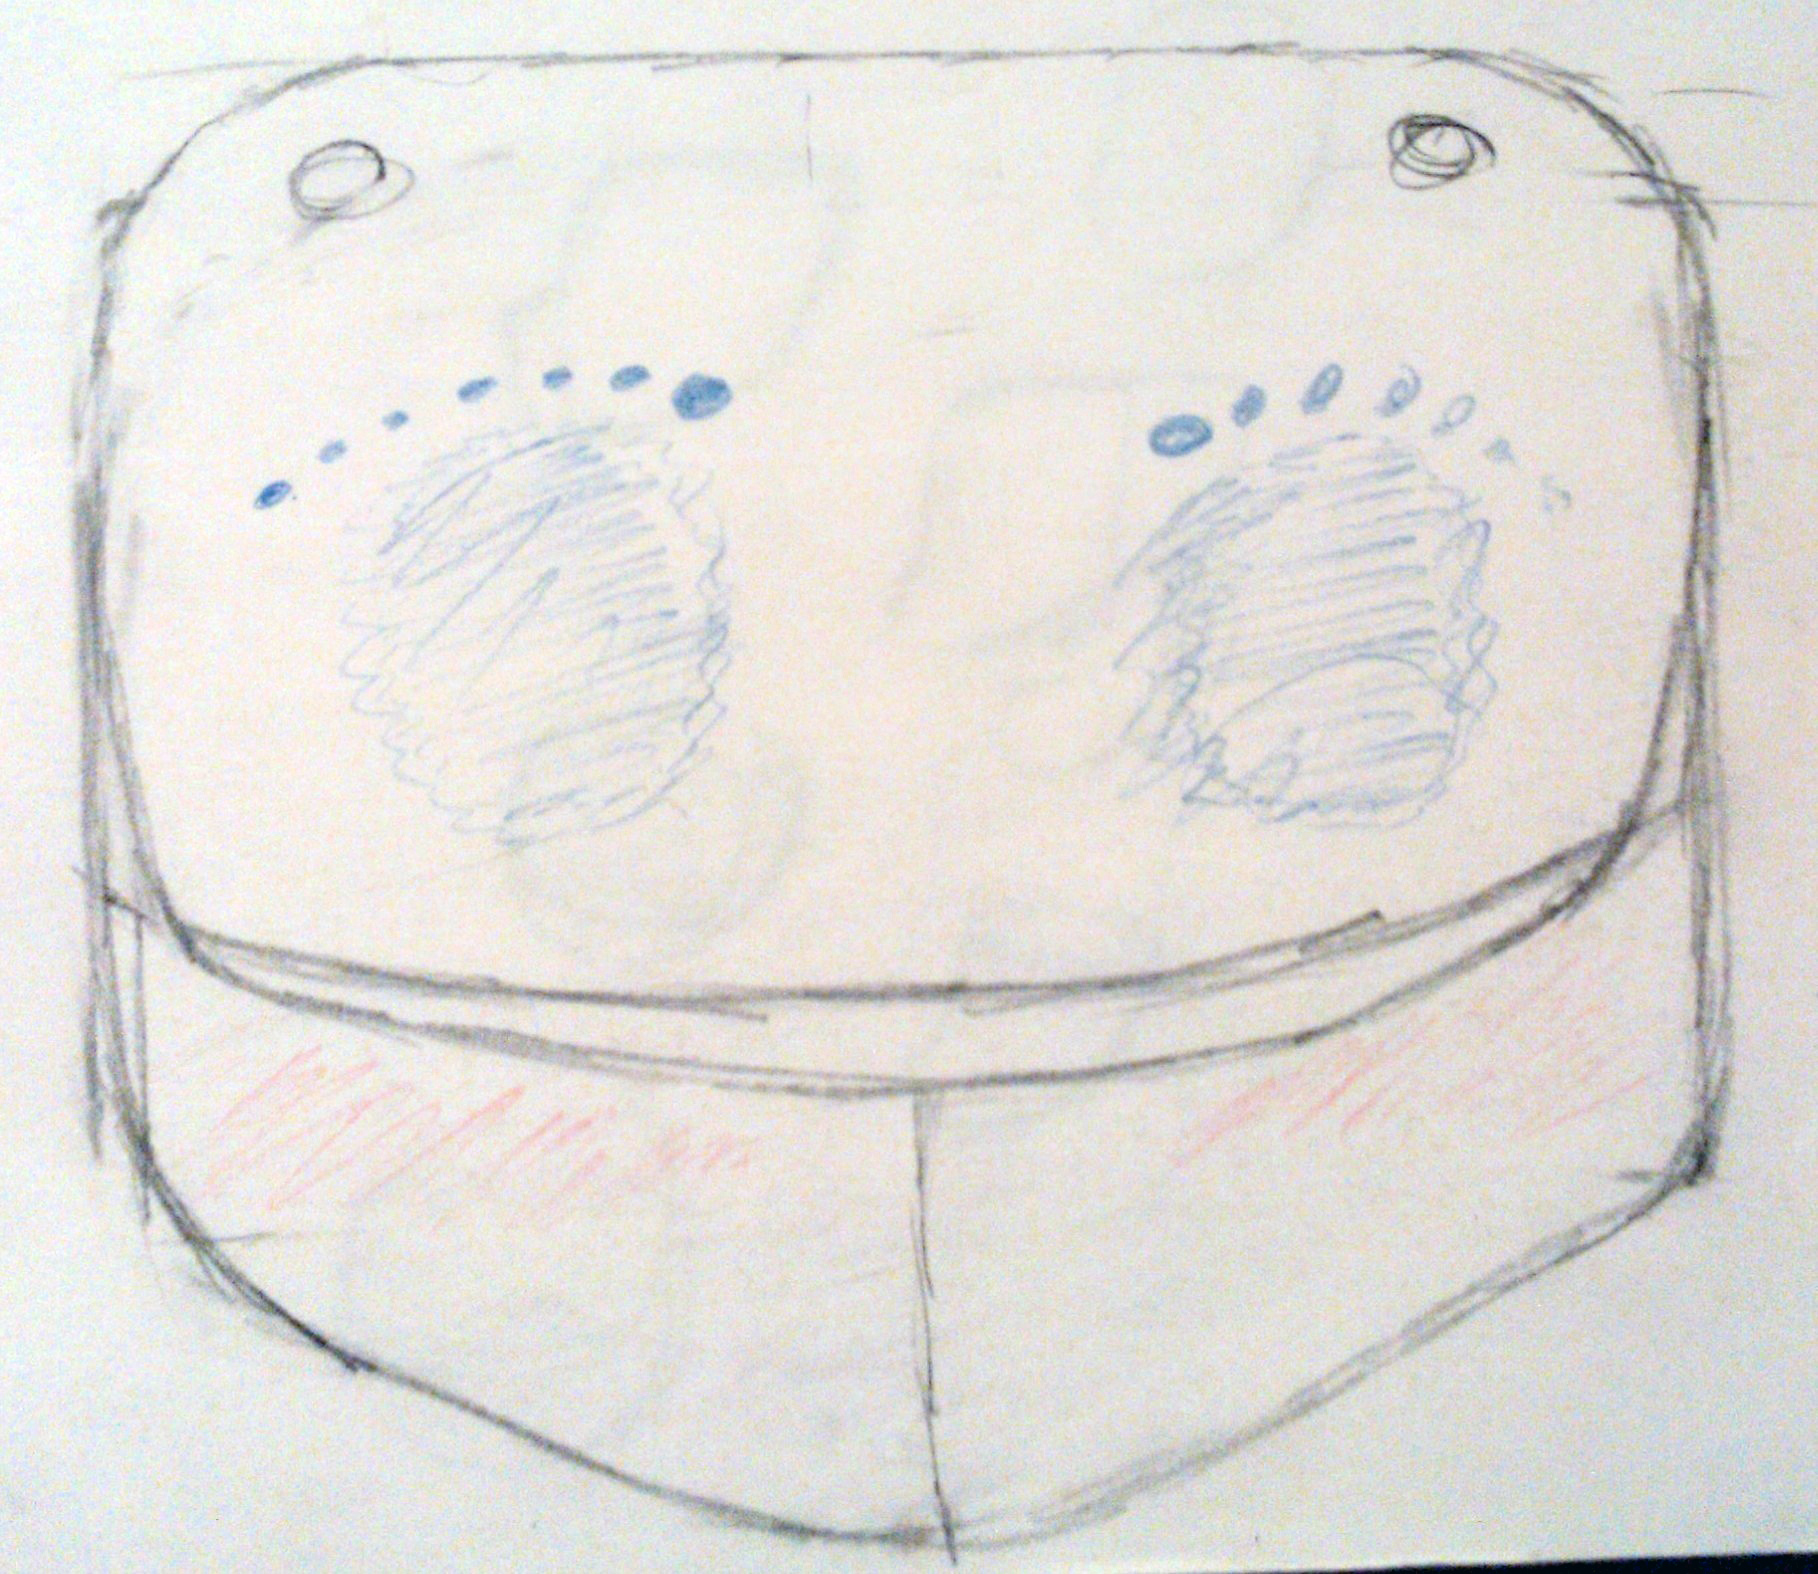
\includegraphics[height=4.5cm]{poppy_head_sketch.jpg}}
    \newline
    \subfloat[][First clay sculpture]{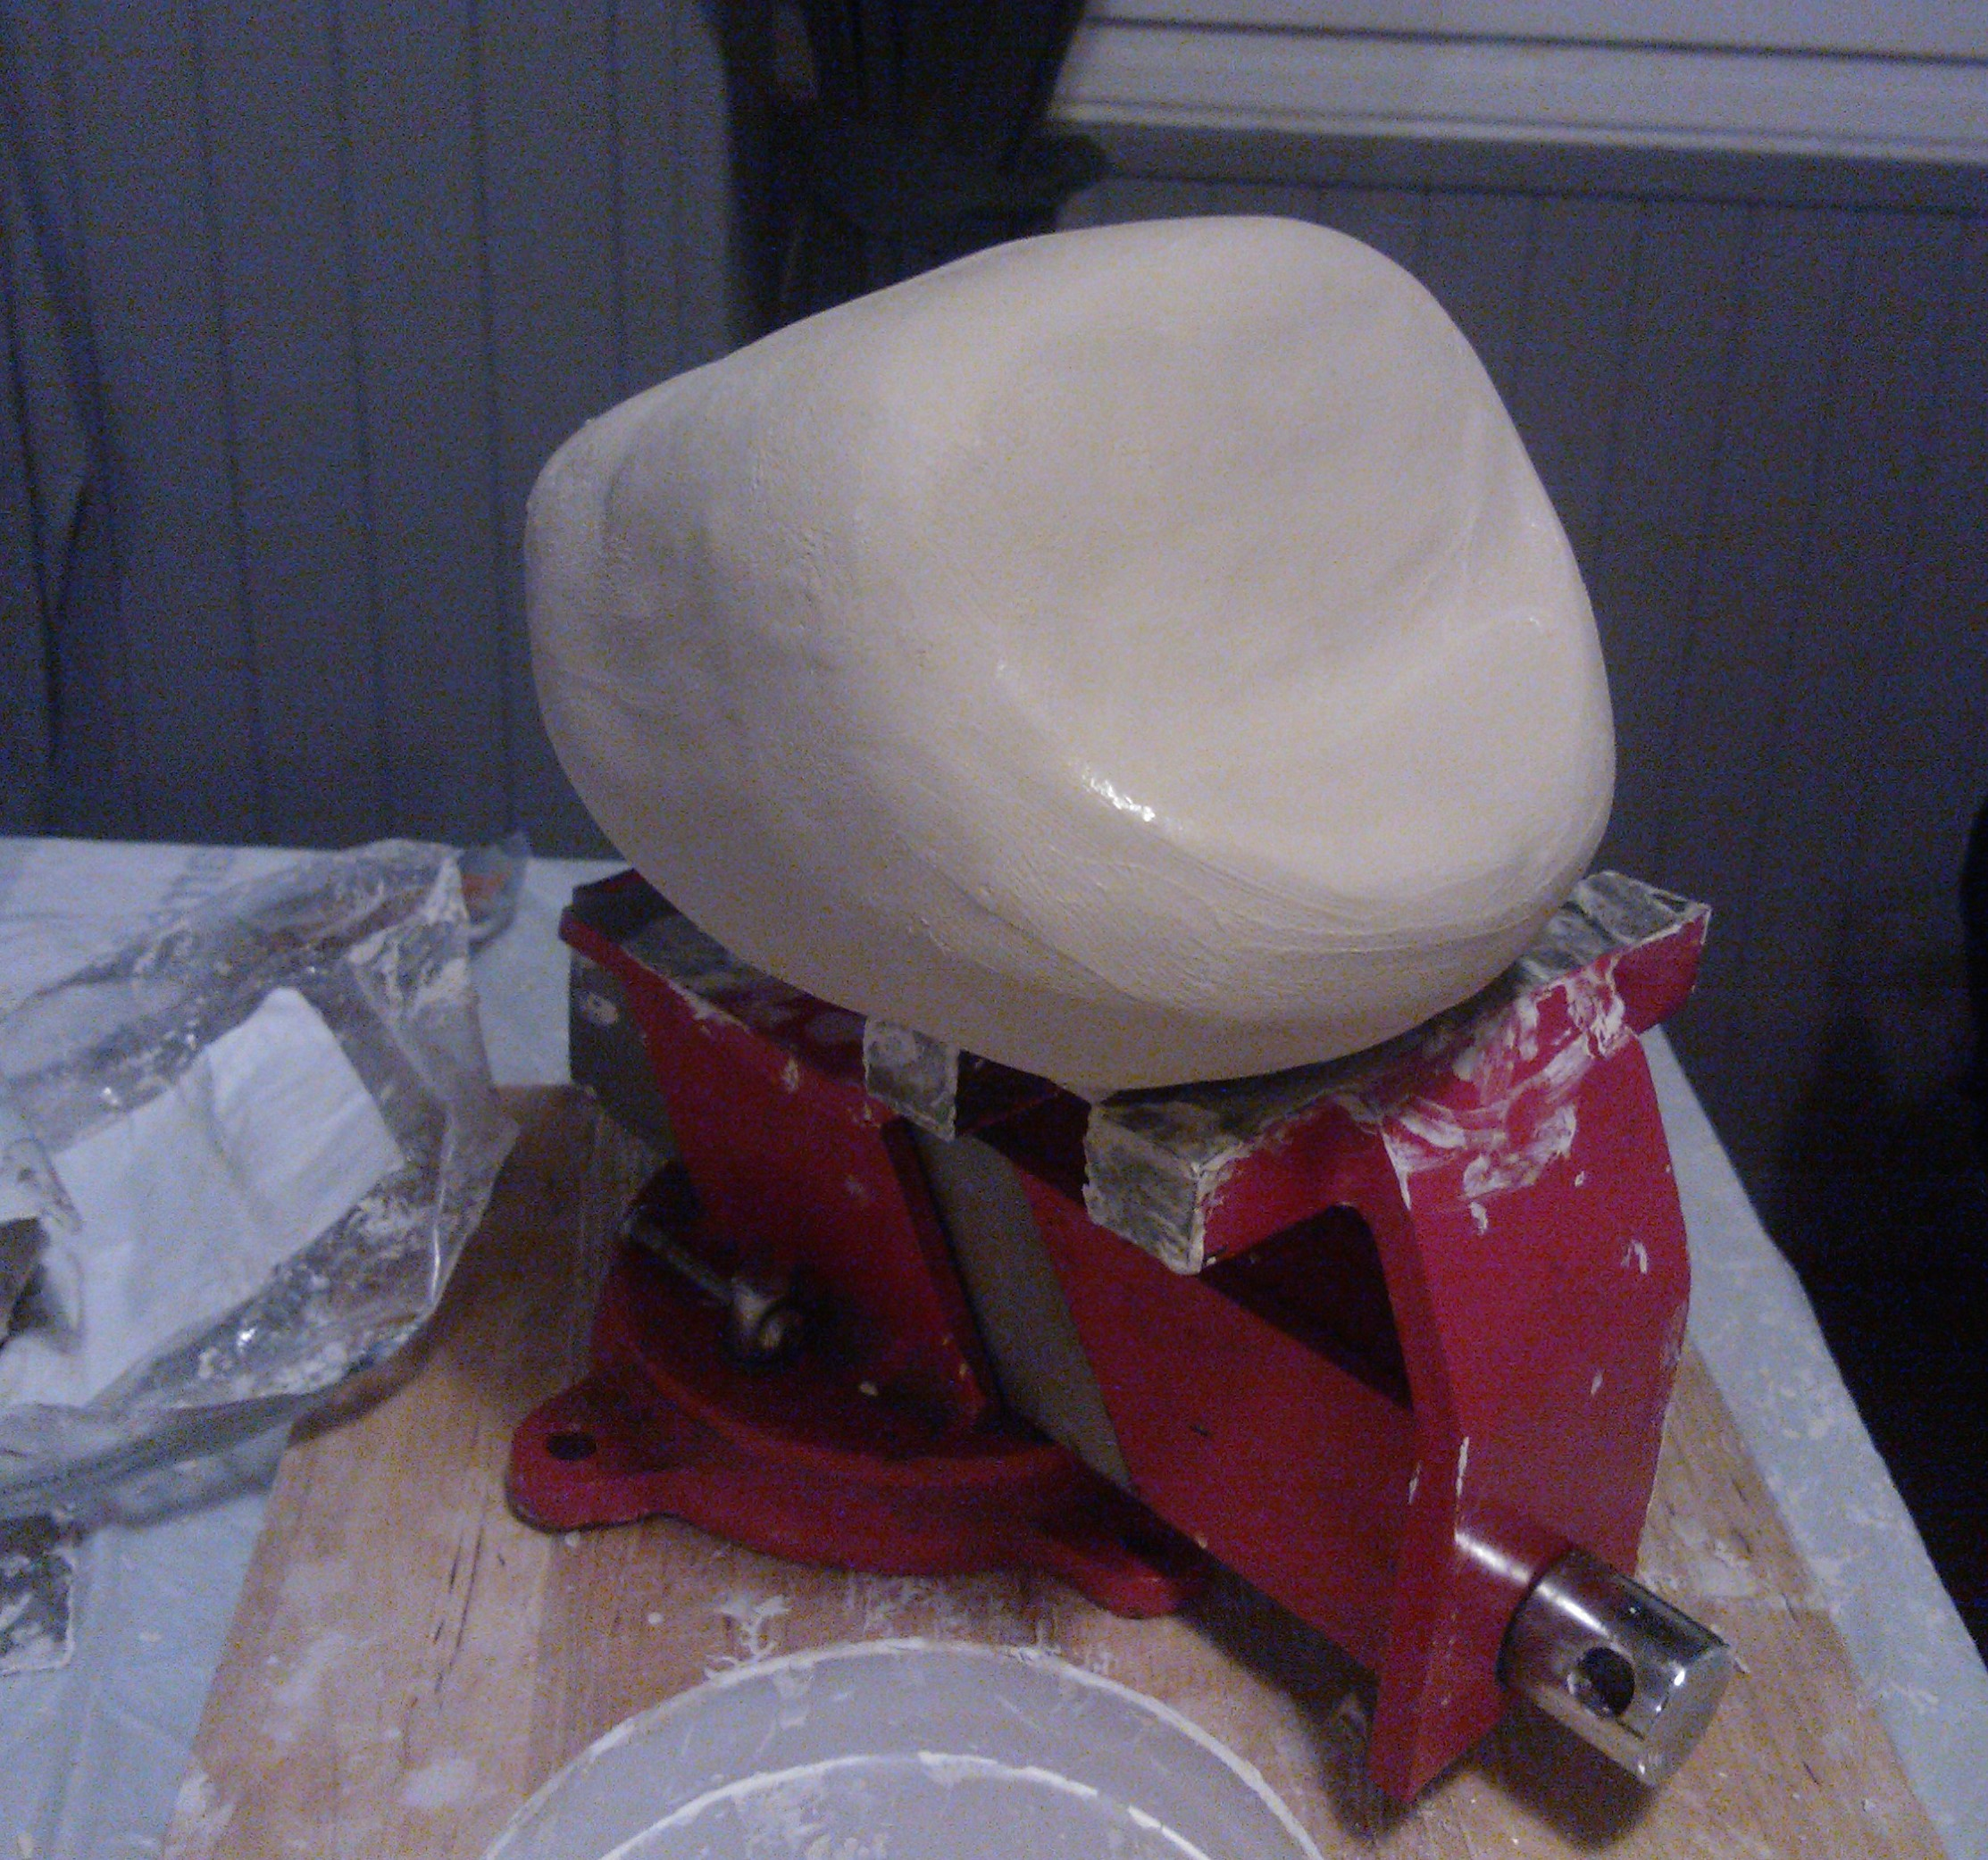
\includegraphics[height=5.5cm]{first_poppy_clay.jpg}}
    \hfil
    \subfloat[][First CAO model]{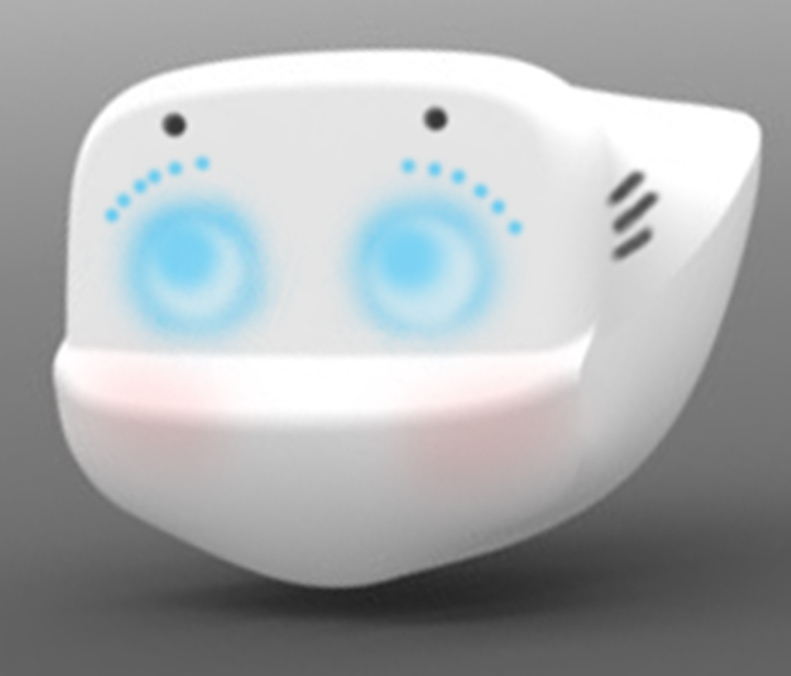
\includegraphics[height=5.5cm]{head_first_trial.jpg}}
    \newline
    \subfloat[][Poppy beta]{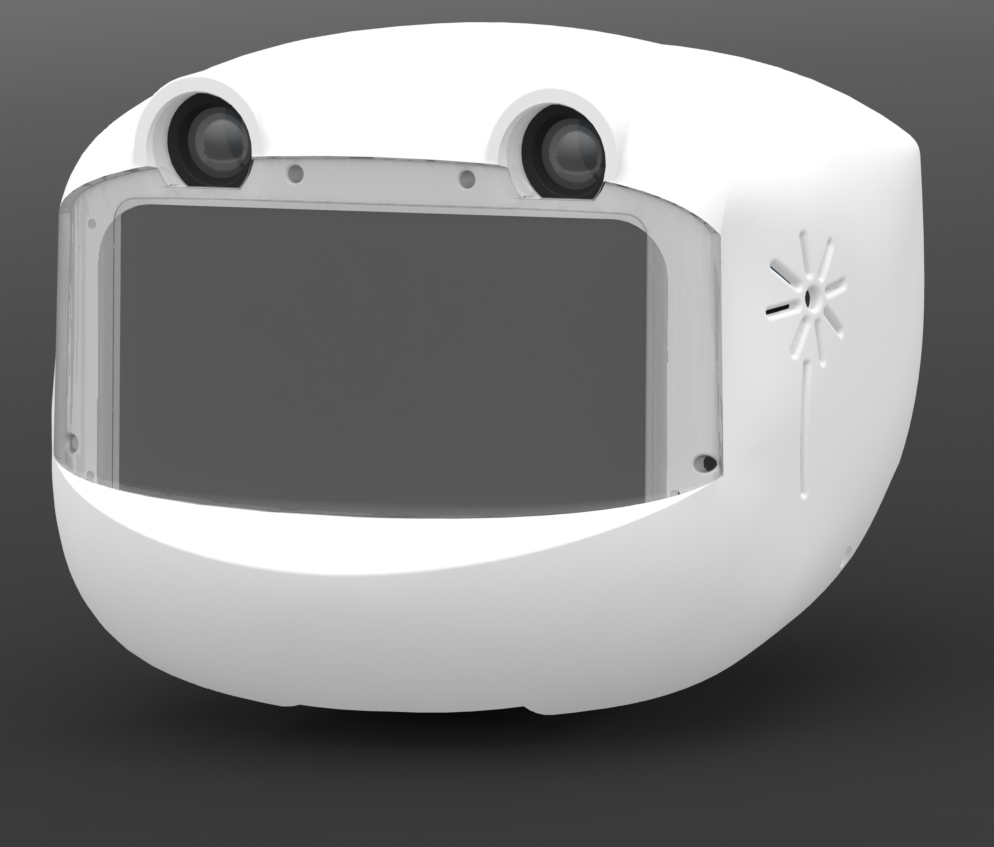
\includegraphics[height=5.5cm]{head_beta.jpg}}
    \hfil
    % \subfloat[][The first assembly]{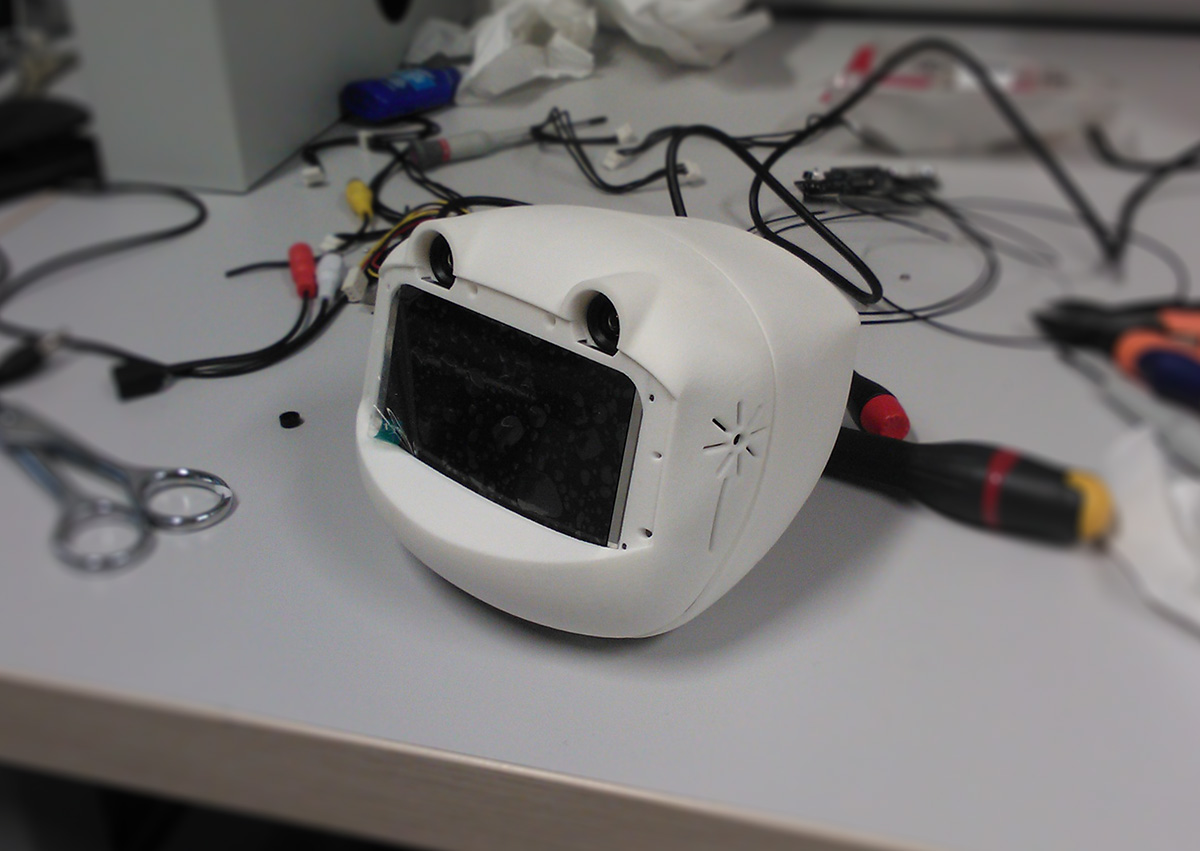
\includegraphics[height=5.5cm]{head_beta_assembled.jpg}}
    % \hfil
    \subfloat[][Screen switched on with basic eyes display]{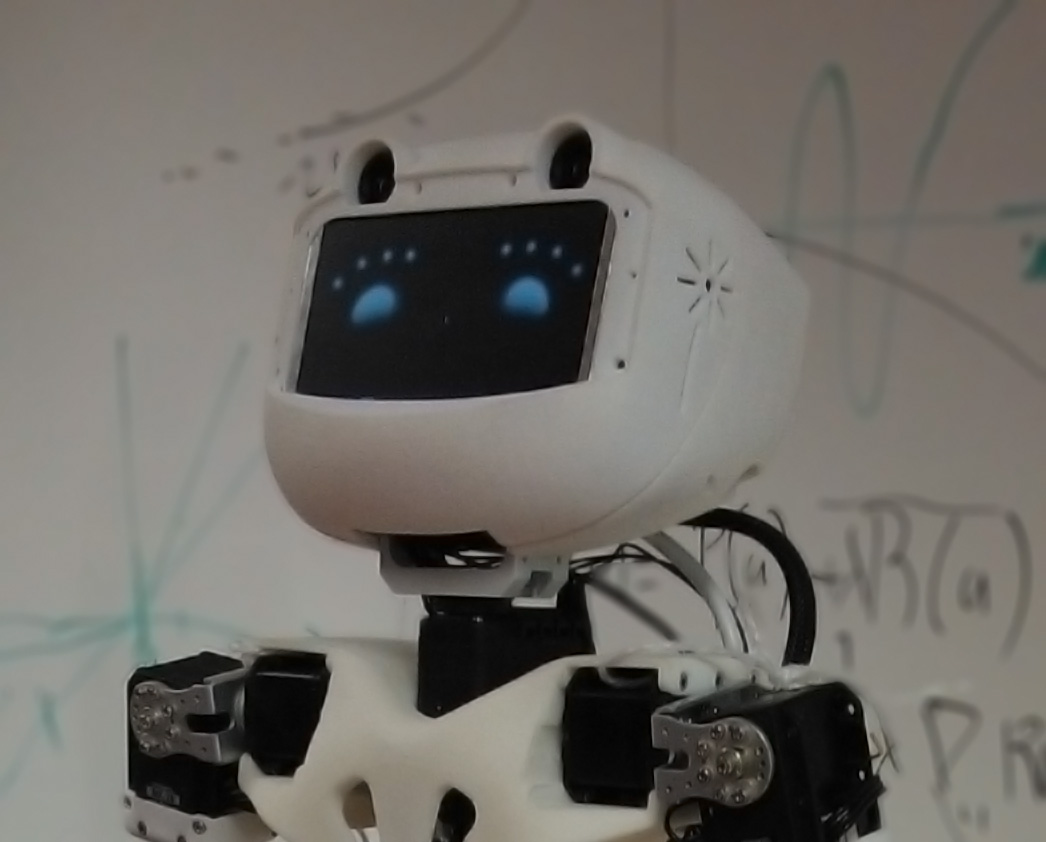
\includegraphics[height=5.5cm]{poppy_beta_eyes.jpg}}
    \caption{Evolution of Poppy’s head from the first sketches to the Poppy beta version.}
    \label{fig:head_sketch}
\end{figure}


However, in the first beta version showed in \figurename~\ref{fig:head_sketch}, there is a major design error. Indeed our desire was to have a screen to create and explore freely expressive eyes but the use of two visible cameras changed the way people saw Poppy's head. Of course, when people see two cameras they consider them to be the eyes of the robot and therefore extrapolate that the screen may be the mouth or another face part.

We are currently working on the new design of Poppy's head and we simply addressed this issue by replacing the two big camera by a small one with a pinhole lens, which can be hidden on Poppy’s face see \figurename~\ref{fig:poppy_head_v1}.

\begin{figure}[tb]
\centering
    % \subfloat[][Mix between Poppy beta 3D printed head and clay sculpture]{\includegraphics[height=5cm]{second_poppy_clay.jpg}}
    % \newline
    \subfloat[][Poppy 1.0]{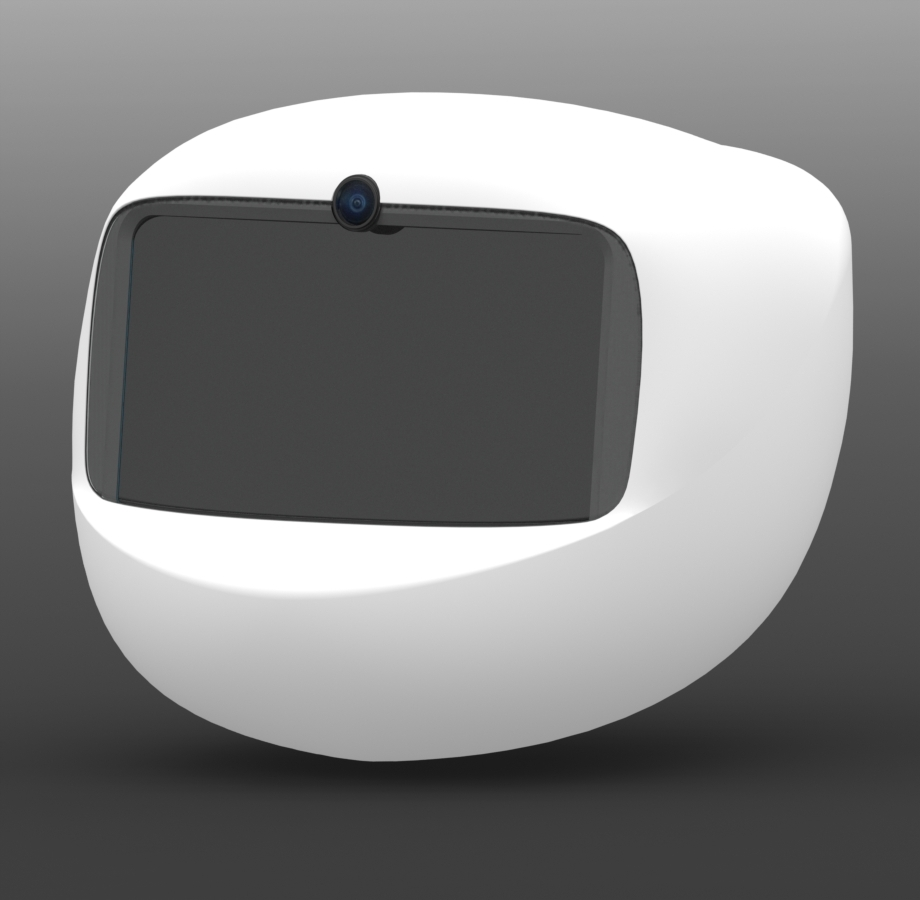
\includegraphics[width=0.5\linewidth]{poppy_v1_head.jpg}}
    \caption{}
    \label{fig:poppy_head_v1}
\end{figure}


While this work it is still in progress, we will update this section afterwards with a blueprint of the electronic integration and final design explanation.
